\providecommand{\main}{../../..}
\documentclass[\main/dresen_thesis.tex]{subfiles}
\renewcommand{\thisPath}{\main/chapters/theoreticalBackground/magnetism}
\begin{document}
\section{Magnetism}\label{ch:theoreticalBackground:magnetism}

  Classically, magnetic fields are understood to be produced by moving electric charges \cite{Jackson_1999_Class, Blundell_2001_Magne}.
  Within the framework of special relativity, magnetic fields emerge via a Lorentz transformation from the rest frame of an electric charge to a relatively moving one and the propagation and interaction of the magnetic field with charge and current distributions is fully described by Maxwell's equations.
  A central quantity to describe the sources of magnetic fields is the magnetic moment $\vec{\mu}$, which for localized current distribution $\vec{j}(\vec{r})$ is defined by
  \begin{align}
    \vec{\mu} \eq \frac{1}{2} \int \vec{r} \times \vec{j}(\vec{r}) \dint V .
  \end{align}
  In the case of a closed loop of current $I$, the magnetic moment is just given by the product of the current and the enclosed area $A$, $\mu \eq I A$, with the direction pointing parallel to the surface normal.
  The far-field generated by a magnetic moment is then given by the dipolar field
  \begin{align}\label{eq:theoreticalBackground:magnetism:dipolarField}
    \vec{B} (\vec{r}) \eq \frac{\mu_0}{4 \pi} \frac{3(\vec{\mu} \cdot \hat{r})\hat{r} - \vec{\mu}}{r^3}.
  \end{align}

  To understand the magnetism of matter, which is generally neutrally charged on the macroscopic scale, the motion of the electrons in the atoms needs to be evaluated\footnote{the direct contribution of the nucleus motion to the magnetism is approximately three orders of magnitude weaker due to the higher mass of the proton and neutrons relative to the electron}.
  The magnetic moment of an electron arises from the spin and orbital motion, which depends on the state the individual particle is in.
  Due to the quantum mechanical nature of the electron, the magnetic moment also needs to be treated quantum mechanically, where it is given for a bound electron by the sum of the operators for the orbital motion and the spin \cite{Coey_2010_Magne}
  \begin{align}
    \vec{\mu}_e \eq \gamma (\vec{L} + g_S \vec{S}),
  \end{align}
  with $\gamma \eq -e/2m_e$ the gyromagnetic ratio and $g_S \eq 2.00231930436146(56)$ the g-factor that is determined to high precision theoretically and experimentally \cite{Aoyama_2012_Tenth, Hanneke_2011_Cavit}.
  In fact, the Bohr-van-Leeuwen theorem shows that for a purely classical system in thermal equilibrium, the magnetization is always zero.
  The various types of magnetism that are observed within different materials in nature can then be understood by the different structures and the effective couplings of the electrons, which in turn determines the direction of the many magnetic moments within the matter.
  The most popular types that are observed throughout this work are described in the following.

  \subsection{Diamagnetism}
    Diamagnetism is a weak effect that is exhibited by every material and measurable when it is not overshadowed by another type of magnetism.
    When a material enters a magnetic field, Faraday's law of induction states that currents are induced, which by Lenz's law are counter directed to the external field.
    For materials with $n$ electrons per volume, the diamagnetic magnetization can be described quantum mechanically in first order perturbation theory by the Langevin diamagnetism \cite{Blundell_2001_Magne}
    \begin{align}
      M \eq \underbrace{- \frac{n e^2}{6 m_e} \braket{r^2}}_{\eq \chi_D} B,
    \end{align}
    where $\braket{r^2}$ is the mean square distance of the electrons from the nucleus.
    The diamagnetic susceptibility $\chi_D$ is always negative and for common materials $\mu_0 \chi_D$ is in the order of $10^{-5}$.

    In magnetometry experiments, diamagnetism is observed from non-magnetic background materials such as a silicon substrate that carries the actual sample of interest or a solvent.
    As the Langevin diamagnetism is a linear function in $B$ that is largely temperature independent, it can in general be easily separated from other magnetic contributions if it is not negligible in strength.

  \subsection{Paramagnetism}\label{ch:theoreticalBackground:magnetism:paramagnetism}
    Paramagnetism is observed in materials that have atomic or molecular orbitals with unpaired electrons.
    At zero field, if the magnetic moments are localized and decoupled, the direction of the moments is randomly distributed through thermal movement.
    Given an external magnetic field, the magnetic moments of the electrons feel a torque that tries to align the electron moment and field to minimize the Zeeman energy
    \begin{align}
      E_Z = - \vec{\mu}_e \cdot \vec{B}.
    \end{align}
    To determine the magnetization of a paramagnetic material at finite temperature and fields, Boltzmann statistics can be applied to obtain the partition function of the system and from this the magnetization.
    In the classical approach, this leads to the formula for Langevin paramagnetism as shown in \refapp{ch:appendix:calculations:magnetizationClassicalSpin}
    \begin{align}
      M \eq n \mu_e \Biggl( \coth \biggl(\frac{\mu_e B}{k_B T} \biggr) - \frac{k_B T}{\mu_e B} \Biggr).
    \end{align}
    For electrons, the energy scale of the Zeeman levels is $\mu_e B \ll k_B T$ and the magnetization is approximated in first order to
    \begin{align}
      M \approx \underbrace{\frac{n \mu_e^2}{3k_B T}}_{\eq \chi_P} B,
    \end{align}
    which shows that the paramagnetic susceptibility is positive and has a temperature dependance according to the Curie law $M \propto T^{-1}$.

  \subsection{Ferromagnetism, Antiferromagnetism, Ferrimagnetism}
    \begin{figure}[tb]
      \centering
      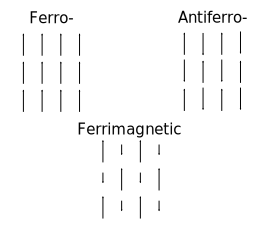
\includegraphics{magnetism_fm_afm}
      \caption{\label{fig:theoreticalBackground:magnetism:fm_afm_fim}Depiction of relative orientation and magnitude of the magnetic moments in a ferro-, antiferro- and ferrimagnetic material.}
    \end{figure}

    When a material has atoms with electrons in an unpaired state nearby to each other, they generally interact for multiple reasons that are touched in the following.
    If the interaction is not negligible, the magnetic moments affect the direction of one another and align mutually along preferred directions.
    \subsubsection{Exchange Interaction}
      A strong quantum mechanical effect between the spin of two electron, the exchange interaction, emerges from the Coulomb interaction and the Pauli exclusion principle.
      Electrons with overlapping states alter their charge distribution by aligning their spins $\vec{S}$ to one another and thus reduce their respective repulsion and the total energy of the system.
      This can effectively expressed by minimizing the exchange energy given by the Heisenberg model
      \begin{align}
        E_{ex} \eq -\sum_{i \neq j} J_{ij} \vec{S}_i \cdot \vec{S}_j,
      \end{align}
      where $J_{ij}$ is the exchange integral that determines the coupling strength between two electron spins.
      Depending on the sign of $J_{ij}$, the energy is minimized by parallel alignment ($J_{ij} > 0$) or anti-parallel alignment ($J_{ij} < 0$).
      The parallel alignment is associated with a ferromagnetic state of the material, whereas the anti-parallel alignment is, when the coupled magnetic moments are of the same magnitude, known as the antiferromagnetic.
      The ferrimagnetic state as depicted in \reffig{fig:theoreticalBackground:magnetism:fm_afm_fim} can be found in mixed compounds, when the anti-parallel aligned moments are not of equal magnitude and therefore a non-zero magnetic moment remains in the net sum.

    \subsubsection{Magnetic Anisotropy}
      Even though the Heisenberg model captures the alignment between magnetic moments, it is isotropic and does not describe observed anisotropies in magnetic materials.
      Due to spin-orbit coupling and dipole-dipole interaction between the electrons, the shape and crystal structure of a material influences the magnetic behaviour and makes some direction in the crystal energetically favorable to another.
      Along this direction, called the easy axis, the magnetization of the material increases stronger than along another direction, whereas the saturation magnetization reached at high fields is independent of the direction.
      The anisotropy can be expressed phenomenological as power series in the directional cosines between the easy-axis and the direction of the magnetization in dependence of the the crystal system.

      In this work, uniaxial and cubic anisotropies are considered.
      The uniaxial system is used to describe a single preferred direction as easy axis or when higher order terms in the anisotropy are negligible.
      If $\theta$ describes the angle between the easy-axis and the magnetization, the anisotropy energy is
      \begin{align}
        E_\mathsf{ani.} \eq K V \sin(\theta)^2,
      \end{align}
      with $K$ the material-dependent anisotropy energy density and $V$ the volume of the material.

      For cubic crystal systems, the anisotropy energy is given by
      \begin{align}
        E_\mathsf{ani.} \eq
          \frac{K_1 V}{4} \biggl(\sin(2 \theta)^2 + \sin(\theta)^4 \sin(2\phi)^2 \biggr) +
          \frac{K_2 V}{16} \biggl( \sin(2 \theta)^2 \sin(2 \phi)^2 \sin(\theta)^2 \biggr),
      \end{align}
      where $\phi, \, \theta$ are the angle between the (001) direction and the magnetization direction in spherical coordinates.
      For $K_1 > 0$ and $K_2 > -9 K_1$ the \{100\} directions of the cubic system are the easy axis and for other values either \{110\} or \{111\} are the easy-axis, depending on the ratio of $K_1$ and $K_2$.

    \subsubsection{Magnetostatic Self-Energy}
      An extended magnetic material produces a stray field, which adds a magnetostatic self-energy to the system that counteracts the magnetization.
      The demagnetizing field $\mu_0 \vec{H}_d$ depends on the shape of the magnet and can be calculated for a given sample magnetization $M$ on the mesoscopic scale using the macroscopic Maxwell's equations of magnetostatics and the material equation, which for a current-free magnetic material are \cite{Jackson_1999_Class}
      \begin{align}
        \vec{\nabla} \cdot \vec{B} \eq& 0,\\
        \vec{\nabla} \times \vec{H} \eq& 0,\\
        \vec{B} \eq& \mu_0 (\vec{H} + \vec{M}).
      \end{align}
      As the magnetic field $H$ is curl-free, it can be expressed by a scalar potential $\vec{H} \eq -\vec{\nabla} U$ according to the Helmholtz theorem.
      Using the material equation and plugging both into the divergence-free condition for the magnetic field $B$, the scalar potential is determined by the differential equations
      \begin{align}
        U \eq \begin{cases}
          \vec{\nabla} \cdot \vec{M}, & \vec{r} \in V \\
          0, &\vec{r} \notin V,
      \end{cases}
      \end{align}
      inside and outside of the magnetic material, with the boundary condition that $U$ and normal component of $B$ is continuous at the surface
      \begin{align}
        U_\mathsf{in} &\eq U_\mathsf{out},\\
        \frac{\partial}{\partial n} U_\mathsf{in} &\eq \frac{\partial}{\partial n} U_\mathsf{out} + \vec{M} \cdot \vec{n}.\\
      \end{align}
      The magnetostatic self-energy is then given by the interaction of the magnetization of the material with the demagnetizing field
      \begin{align}
        E_{ms} \eq -\frac{\mu_0}{2} \int_V \vec{M} \cdot \vec{H}_d \dint V
      \end{align}
      To minimize the magnetostatic energy, it becomes above a material-dependent crystallite volume energetically favorable to create separate domains of regions with coherent spin alignment and therefore vary the magnetization direction across the material.
      The average domain size is then determined by the balance of energy needed to keep the domain walls and the energy gained from minimizing the self-energy.

    The domain formation and the magnetic anisotropy both result in the characteristic hysteretic magnetization behaviour observed for ferromagnetic and ferrimagnetic bulk materials below the order temperature.
    % Upon exposure to a sufficiently strong external magnetic field a hyst, with a remanent magnetization $M_R$ at removal of the field and the need of a coercive field $B_C$ to return the magnetization of the material to zero.

  \subsection{Superparamagnetism}
    When the crystallite size of a ferro- or ferrimagnetic material is reduced, domain formation is no longer energetically favorable below a material-dependent size, which is typically in the order of nanometers.
    At this point, the individual electron magnetic moments in the crystallites can align to one another in a single domain via the exchange interaction and add to a coherent superspin.
    If the thermal energy is high enough to overcome the energy barrier from the magnetic anisotropy, the superspin of the single domain can freely rotate and the material is said to be in a superparamagnetic phase.
    In this magnetic phase, no hysteresis is observed, but the material still shows a large magnetization, comparable to the ferromagnetic state, when exposed to an external magnetic field.
    The magnetization for an ensemble of monodisperse and non-interacting superparamagnetic particles can be described by the same Langevin function, which is used in paramagnetism
    \begin{align}
      M \eq M_s \Biggl( \coth \biggl(\frac{\mu B}{k_B T} \biggr) - \frac{k_B T}{\mu B} \Biggr),
    \end{align}
    where this time $\mu$ is the magnetic moment of the individual particle and $M_s \eq \mu / V_p$ is a material-dependent constant.
    Due to additional surface effects and possible disorder in the nanoparticle, the nanoparticle $M_s$ of a specific material does not need to coincide with the bulk value.

    The time scale at which a particle superspin flips by overcoming the anisotropy energy barrier due to thermal motion is called the N\'eel relaxation time $\tau_N$ and given for uniaxial particles by the N\'eel-Arrhenius equation
    \begin{align}
      \tau_N \eq \tau_0 \exp \biggl( \frac{KV}{k_B T} \biggr),
    \end{align}
    where $K$ is the material-dependent anisotropy energy density, $V$ the particle volume and $\tau_0$ the attempt time, which is typically in the order of $1 \unit{ps} - 10 \unit{ns}$, depending on the material.

    When the magnetization of a material is measured on a timescale of $\tau_m \gg \tau_N$, the material will show the superparamagnetic magnetization behaviour as the spin flips several times during the measurement.
    If the temperature is lowered such that $\tau_m < \tau_N$, the material will appear to be in a blocked state and show a hysteretic magnetization behaviour.
    The transition temperature, called the blocking temperature, can be determined by setting $\tau_m \eq \tau_N$
    \begin{align}
      \label{eq:theoreticalBackground:superparamagnetism:blockingTemp}
      T_B \eq \frac{KV}{k_B \log(\tau_m/\tau_0)},
    \end{align}
    where for typically $\tau_m \approx 1 \unit{s}$, the value of the logarithm is in the order of $20 - 25$.

    When nanoparticles are free to move in dispersion, another relaxation process is possible by rotational Brownian motion that has a relaxation time of \cite{Einstein_1956_Inves}
    \begin{align}
      \tau_B \eq \frac{3 \eta V}{k_B T},
    \end{align}
    where $\eta$ is the viscosity of the dispersion and $V$ the hydrodynamic volume of the particle.
    This additional degree of freedom makes it possible that even when a nanoparticle can not overcome the anisotropy energy barrier by means of thermal energy that it can change it's magnetic moment direction by a physical rotation in dispersion and therefore under those circumstances aligns itself to an external field for example.

    Superparamagnetic particles present an interesting system to study dipolar magnetic effects.
    In contrast to the atomic length scale where dipolar interaction is negligible in comparison to the exchange interaction, the magnetic moment of a particle $\mu$ is typically four order of magnitudes larger than the magnetic moment of a single electron and dipolar interaction of single domains is therefore still relevant on nanometer length scales.
    As the dipolar field is directional and there is magnetic anisotropy for every domain in the system, the emergent ground state for a system of single domains will highly depend on the choice of material and relative orientation and position of the particles as will be shown.

  \subsection{Modeling Magnetic Nanoparticle Dynamics}
    In this work, ensembles of magnetic nanoparticles are discussed in dispersion, as well as in fixed in nanostructures.
    To understand the magnetic properties observed when external parameters such as the outer magnetic field or the temperature is varied, this section discusses the basics for the simulation of nanoparticle dynamics in principle.
    The results are helpful to understand the relevant timescales and how to calculate at which parameter ranges effects emerging from specific contribution are expected to be observed.

    As discussed, the energy of a system of magnetic nanoparticles can be modeled on the atomic level as a sum of the exchange interaction, the magnetic anisotropy, the interaction between the particles that is assumed to be dipolar, the interaction with an external field and possibly further microscopic degrees of freedom that appear random on the macroscopic scale and are summarized as noise
    \begin{align}
      E \eq E_\mathsf{ex.} + E_\mathsf{ani.} + E_\mathsf{dip.-dip.} + E_\mathsf{ext.} + E_\mathsf{noise},
    \end{align}
    A general approach to minimize this energy is either to perform Monte Carlo simulations or to use the stochastic Landau-Lifshitz-Gilbert (LLG) equation \cite{Fidler_2000_Micro, Scholz_1999_Micro} for atomistic magnetic spins $\vec{S}_i$
    \begin{align}
      \frac{\dint \hat{S}_i}{\dint t} \eq
        - \frac{\gamma}{1 + \alpha^2} \biggl(
          \hat{S}_i \times (\vec{B}_i^\mathsf{eff.} + \vec{B}^\mathsf{therm.}_i) +
          \alpha \hat{S}_i \times \bigl(\hat{S}_i \times (\vec{B}_i^\mathsf{eff.} +\vec{B}^\mathsf{therm.}_i) \bigr) \biggr),
    \end{align}
    where the associated magnetic fields are obtained via the thermodynamic relation
    \begin{align}
      \vec{B}_i \eq - \frac{\dint E}{\dint \vec{S}_i},
    \end{align}
    which add up to an effective field
    \begin{align}
      \vec{B}^\mathsf{eff.}_i \eq \vec{B}^\mathsf{ex.}_i + \vec{B}^\mathsf{ani.}_i + \vec{B}^\mathsf{dip.-dip.}_i + \vec{B}^\mathsf{ext.},
    \end{align}
    and the noise is treated separately as an additional thermal field $\vec{B}^\mathsf{therm.}$.
    The thermal field is assumed to be uncorrelated in time and space and to follow a Gaussian stochastic process due to the central limit theorem.
    The first and second moment of the random variables are thus assumed to be
    \begin{align}
      \braket{B^\mathsf{therm.}_i (t)} &\eq 0,\\
      \braket{B^\mathsf{therm.}_i (t) B^\mathsf{therm.}_j (t^\prime)} &\eq 2 D \delta_{ij} \delta(t - t^\prime),
    \end{align}
    with the diffusion coefficient $D$ determined by studying the stationary solutions of the Fokker-Planck equation associated with the stochastic LLG equation to \cite{Garcia_1998_Lange}
    \begin{align}
      D \eq \frac{\alpha}{1 + \alpha^2} \frac{k_B T}{\gamma M_S V}.
    \end{align}
    In the LLG equation, $\gamma$ is the electron gyromagnetic ratio, which is for a electron spin system $\gamma \eq 0.1760859644(11) \unit{ps^{-1} T^{-1}}$, and $\alpha$ the Gilbert damping constant that is typically in the range of $\alpha \eq 0.01 \ldots 1$.
    The damping constant is added phenomenologically in the equation to include the observation that after some time, if not disturbed by strong thermal fluctuations, the spins align with the effective field due to internal frictions in the system.
    The evolution of the moments can then finally be determined by numerically integrating the set of differential equations \textit{e.g.} by Heun's method \cite{Sueli_2003_Anint}.

    It is noteworthy that for nanoparticle assemblies this model can become large rather quick as every nanoparticle in the assembly has to be modeled by a number of atomistic magnetic moments.
    However, as one is often not interested in the atomistic details, only the evolution of the nanoparticle superspins is of interest.
    Applying the LLG equation directly to macroscopic spins has some drawbacks in the implementation of thermal effects, as it models only coherent rotations of the superspin with constant magnitude and does not include spin wave dispersion.
    For this purpose, the stochastic Landau-Lifshitz-Bloch (LLB) equation \cite{Evans_2012_Stoch, Atxitia_2017_Funda} has been developed as extension to describes the mesoscopic evolution of spins coupled on the mesoscopic scale by their exchange interaction such as in the case of nanoparticles. For macroscopic magnetic moment $\vec{\mu} \eq \vec{M} / M_S^0$ that are normalized to their saturation value at $T \eq 0$ it reads
    \begin{align}
      \frac{\dint \vec{\mu}_i}{\dint t} \eq
        - \gamma \biggl(
          \vec{\mu}_i \times \vec{B}_i^\mathsf{eff.} -
          \frac{\alpha_\parallel}{\mu^2} \bigl(\vec{\mu}_i \cdot \vec{B}_i^\mathsf{eff.} \bigr) \vec{\mu}_i +
          \frac{\alpha_\bot}{\mu^2} \vec{\mu}_i \times \bigl(\vec{\mu}_i \times (\vec{B}_i^\mathsf{eff.} + \vec{B}^\mathsf{therm.}_{i, \, \bot}) \bigr) +  \vec{B}^\mathsf{therm.}_{i, \, ad} \biggr),
    \end{align}
    This modified differential equation introduces an additional term, damping factor and stochastic variable.
    It was demonstrated that this equation reproduces the Boltzmann distribution and can be applied to nanoparticles at high temperatures.

    A full implementation and analysis of the discussed systems via either the stochastic LLG or LLB equations goes beyond the scope of this work.
    However, the relevant magnetic field strengths and therefore temperature and time scales can still be estimated from this theory and is discussed in their respective chapters.
    In the following, we list the equations needed to determine the fields from the magnetic anisotropy and dipole-dipole interaction energy.

    For uniaxial and cubic anisotropy, the anisotropy field of a nanoparticle is given by
    \begin{align}
      \vec{B}^\mathsf{ani.}_{i, \,\mathsf{uniaxial}} &\eq \frac{2 K V}{\mu} \bigl( \hat{\mu}_i \cdot \hat{n} \bigr) \hat{n},\\
      \vec{B}^\mathsf{ani.}_{i, \,\mathsf{cubic}} &\eq \frac{2 V}{\mu} \begin{pmatrix}
        K_1 (\hat{\mu}_{i, x}^2 - 1) \hat{\mu}_{i, x} - K_2 (\hat{\mu}_{i, y} \hat{\mu}_{i, z})^2 \hat{\mu}_{i, x} \\
        K_1 (\hat{\mu}_{i, y}^2 - 1) \hat{\mu}_{i, y} - K_2 (\hat{\mu}_{i, x} \hat{\mu}_{i, z})^2 \hat{\mu}_{i, y} \\
        K_1 (\hat{\mu}_{i, z}^2 - 1) \hat{\mu}_{i, z} - K_2 (\hat{\mu}_{i, x} \hat{\mu}_{i, y})^2 \hat{\mu}_{i, z}
      \end{pmatrix},
    \end{align}

    The dipole-dipole field is evaluated for each particle by summing the dipole fields produced by the other superspins
    \begin{align}
      \vec{B}^\mathsf{dip.-dip.}_i \eq \frac{\mu \mu_0}{4 \pi}  \sum_{i \neq j} \frac{3 \hat{r}_{ij}  (\mu_j \cdot \hat{r}_{ij}) - \mu_j}{r_{ij}^3},
    \end{align}
    with $\hat{r}_{ij}$ the unit vector describing the direction from the position of $\mu_j$ to $\mu_i$ and $r_{ij}$ the magnitude of the distance.

    

    % \subsubsection{Single Particle}
    %   In the case of a single nanoparticle, the dipole-dipole interaction term can be omitted and the energy is determined by anisotropy, thermal and the external field.
    %   When the temperature is set to zero and the particle considered to have an uniaxial anisotropy, the model is known as the Stoner-Wohlfarth model.


    % hier weiter
    % The numerical implementation is then performed in \textsc{Fortran90} by initializing first a system of magnetic moments, tabulating their respective positions and distances to one another, and then evolving the system in discrete time steps by recursively applying Heun's method \cite{Sueli_2003_Anint} to the set of ordinary differential equations.
    % Random gaussian numbers needed for the simulation of thermal noise are generated using the Box-Mueller transform \cite{Box_1957_Anoteo}.
    % After each time step, the magnetic moment vector directions $\hat{\mu}$ are normalized to avoid numerical instabilities.


\end{document}